\documentclass[11pt,a4paper]{article}
\usepackage[utf8]{inputenc}
\usepackage{graphicx}
\usepackage{geometry}
\usepackage{listings}
\usepackage{xcolor}
\usepackage{hyperref}
\usepackage{float}

% Margins
\geometry{
 a4paper,
 total={170mm,257mm},
 left=20mm,
 top=20mm,
}

% Code Listing Style
\definecolor{codegreen}{rgb}{0,0.6,0}
\definecolor{codegray}{rgb}{0.5,0.5,0.5}
\definecolor{codepurple}{rgb}{0.58,0,0.82}
\definecolor{backcolour}{rgb}{0.95,0.95,0.92}

\lstdefinestyle{mystyle}{
    backgroundcolor=\color{backcolour},   
    commentstyle=\color{codegreen},
    keywordstyle=\color{magenta},
    numberstyle=\tiny\color{codegray},
    stringstyle=\color{codepurple},
    basicstyle=\ttfamily\footnotesize,
    breakatwhitespace=false,         
    breaklines=true,                 
    captionpos=b,                    
    keepspaces=true,                 
    numbers=left,                    
    numbersep=5pt,                  
    showspaces=false,                
    showstringspaces=false,
    showtabs=false,                  
    tabsize=2
}

\lstset{style=mystyle}

\title{GreenTrack Project Submission Report}
\author{Amit Kumar Jha (24BCE5082) \\ Aryan Patel (24BCE5048) \\ Abhijay Jha (24BCE5136)}
\date{\today}

\begin{document}

\maketitle
\tableofcontents
\newpage

% --- NEW HANDWRITTEN SECTIONS ---

\section{Abstract of the Project}
\begin{figure}[H]
    \centering
    \framebox[\textwidth]{\rule{0pt}{300pt}\textless PASTE HANDWRITTEN ABSTRACT HERE \textgreater}
\end{figure}
\clearpage

\section{Modules of the Project}
\begin{figure}[H]
    \centering
    \framebox[\textwidth]{\rule{0pt}{400pt}\textless PASTE HANDWRITTEN MODULES DESCRIPTION HERE \textgreater}
\end{figure}
\clearpage

\section{Design of Database}
\begin{figure}[H]
    \centering
    \framebox[\textwidth]{\rule{0pt}{400pt}\textless PASTE HANDWRITTEN DATABASE DESIGN HERE \textgreater}
\end{figure}
\clearpage

% --- EXISTING CONTENT ---

\section{Project Overview}
GreenTrack is a social gamification platform for tree planting, built with React, Node.js, and MySQL. This report documents the database schema, backend logic, and system configuration.

\section{Database Schema (DDL)}
The following SQL commands defined in \texttt{server/schema.sql} are used to structure the MySQL database.

\subsection{Users Table}
Stores user profiles, synchronized with Firebase Authentication.
\begin{lstlisting}[language=SQL]
CREATE TABLE IF NOT EXISTS users (
    uid VARCHAR(128) PRIMARY KEY,
    name VARCHAR(255) UNIQUE, -- Global unique username
    email VARCHAR(255) UNIQUE,
    photo_url TEXT,
    points INT DEFAULT 0,
    level INT DEFAULT 1,
    xp INT DEFAULT 0,
    trees_planted INT DEFAULT 0,
    verified_posts INT DEFAULT 0,
    role VARCHAR(50) DEFAULT 'user',
    community_id VARCHAR(50) DEFAULT 'global',
    community_name VARCHAR(255) DEFAULT 'Global Earth Guardians',
    is_community_leader BOOLEAN DEFAULT FALSE,
    created_at TIMESTAMP DEFAULT CURRENT_TIMESTAMP
);
\end{lstlisting}

\subsection{Trees Table}
Stores the inventory of planted trees. Includes a composite unique key to ensure each user has unique tree tags.
\begin{lstlisting}[language=SQL]
CREATE TABLE IF NOT EXISTS trees (
    id INT AUTO_INCREMENT PRIMARY KEY,
    tree_tag VARCHAR(50) NOT NULL, -- User-defined ID (e.g., GARDEN-01)
    species VARCHAR(255) NOT NULL,
    planted_date DATE,
    location VARCHAR(255),
    caretaker_id VARCHAR(128),
    health_score INT DEFAULT 100,
    created_at TIMESTAMP DEFAULT CURRENT_TIMESTAMP,
    FOREIGN KEY (caretaker_id) REFERENCES users(uid),
    UNIQUE KEY unique_user_tree (caretaker_id, tree_tag) -- Uniqueness Constraint
);
\end{lstlisting}

\subsection{Posts Table}
Stores social feed content (images, captions) linked to users and trees.
\begin{lstlisting}[language=SQL]
CREATE TABLE IF NOT EXISTS posts (
    id INT AUTO_INCREMENT PRIMARY KEY,
    user_id VARCHAR(128),
    user_name VARCHAR(255),
    user_photo TEXT,
    tree_id INT,
    caption TEXT,
    image_url TEXT,
    has_image BOOLEAN DEFAULT FALSE,
    community_id VARCHAR(50),
    location_lat DECIMAL(10, 8),
    location_lng DECIMAL(11, 8),
    status VARCHAR(50) DEFAULT 'verified',
    upvotes_count INT DEFAULT 0,
    created_at TIMESTAMP DEFAULT CURRENT_TIMESTAMP,
    FOREIGN KEY (user_id) REFERENCES users(uid),
    FOREIGN KEY (tree_id) REFERENCES trees(id)
);
\end{lstlisting}

\subsection{Communities and Comments}
\begin{lstlisting}[language=SQL]
CREATE TABLE IF NOT EXISTS communities (
    id VARCHAR(50) PRIMARY KEY,
    name VARCHAR(255),
    leader_id VARCHAR(128),
    FOREIGN KEY (leader_id) REFERENCES users(uid)
);

CREATE TABLE IF NOT EXISTS comments (
    id INT AUTO_INCREMENT PRIMARY KEY,
    post_id INT,
    user_id VARCHAR(128),
    text TEXT NOT NULL,
    created_at TIMESTAMP DEFAULT CURRENT_TIMESTAMP,
    FOREIGN KEY (post_id) REFERENCES posts(id) ON DELETE CASCADE,
    FOREIGN KEY (user_id) REFERENCES users(uid)
);
\end{lstlisting}

\section{Backend Implementation (API Queries)}
Backend logic handled in \texttt{server/index.js}.

\subsection{User Authentication and Sync}
\textbf{Logic:} Verifies Firebase token, checks if user exists in MySQL, and creates a record if new.
\begin{lstlisting}[language=SQL]
-- Check availability
SELECT uid FROM users WHERE name = ?

-- Create User
INSERT INTO users (uid, name, email, photo_url, community_id, community_name) 
VALUES (?, ?, ?, ?, ?, ?)
\end{lstlisting}

\subsection{Tree Registration}
\textbf{Logic:} Registers a tree and ensures the \texttt{tree\_tag} is unique for that user. Awards gamification points.
\begin{lstlisting}[language=SQL]
-- Register Tree
INSERT INTO trees (tree_tag, species, planted_date, location, caretaker_id) 
VALUES (?, ?, ?, ?, ?)

-- Award Points
UPDATE users SET trees_planted = trees_planted + 1, points = points + 20, xp = xp + 20 
WHERE uid = ?
\end{lstlisting}

\subsection{Social Mechanics}
\textbf{Logic:} Handles posting, liking, and commenting.
\begin{lstlisting}[language=SQL]
-- Create Post
INSERT INTO posts (user_id, ... ) VALUES (?, ... )

-- Like Post
UPDATE posts SET upvotes_count = upvotes_count + 1 WHERE id = ?
UPDATE users SET points = points + 1 WHERE uid = ? -- Reward author

-- Fetch Feed
SELECT * FROM posts WHERE tree_id = ? AND community_id = ? 
ORDER BY created_at DESC LIMIT 50
\end{lstlisting}

\section{Entity-Relationship (ER) Diagram}
\begin{figure}[H]
    \centering
    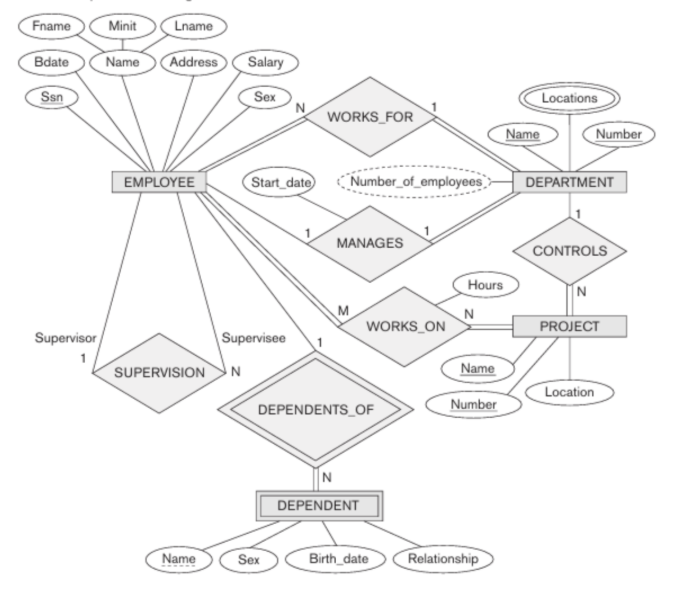
\includegraphics[width=0.9\textwidth]{uploaded_image_1768838443616.png}
    \caption{Hand-drawn Entity-Relationship Diagram}
\end{figure}

\section{System Configuration and Setup}

\subsection{Environment Setup}
Initializing the Node.js server and installing dependencies.
\begin{figure}[H]
    \centering
    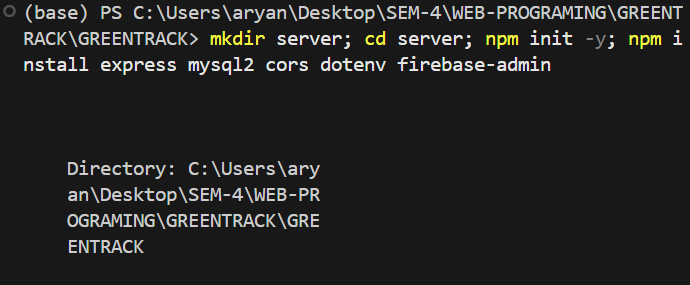
\includegraphics[width=0.9\textwidth]{uploaded_image_0_1768840342969.png}
    \caption{Terminal Setup}
\end{figure}

\subsection{Package Installation}
Successful installation of backend packages.
\begin{figure}[H]
    \centering
    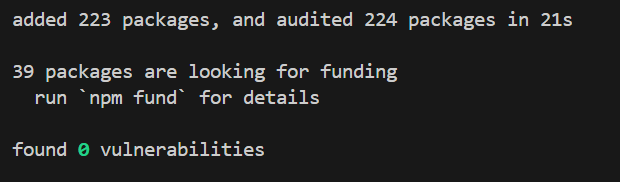
\includegraphics[width=0.9\textwidth]{uploaded_image_1_1768840342969.png}
    \caption{NPM Dependency Installation}
\end{figure}

\subsection{Database Creation}
Executing \texttt{CREATE TABLE} commands in the MySQL CLI.
\begin{figure}[H]
    \centering
    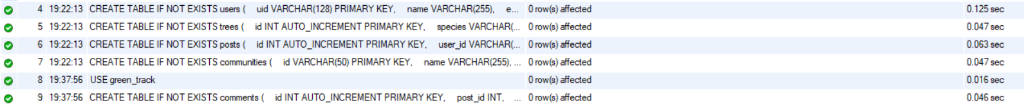
\includegraphics[width=0.9\textwidth]{uploaded_image_2_1768840342969.png}
    \caption{My SQL Schema Verification}
\end{figure}

\subsection{Google OAuth Configuration}
Setting up the OAuth client ID for Firebase Authentication.
\begin{figure}[H]
    \centering
    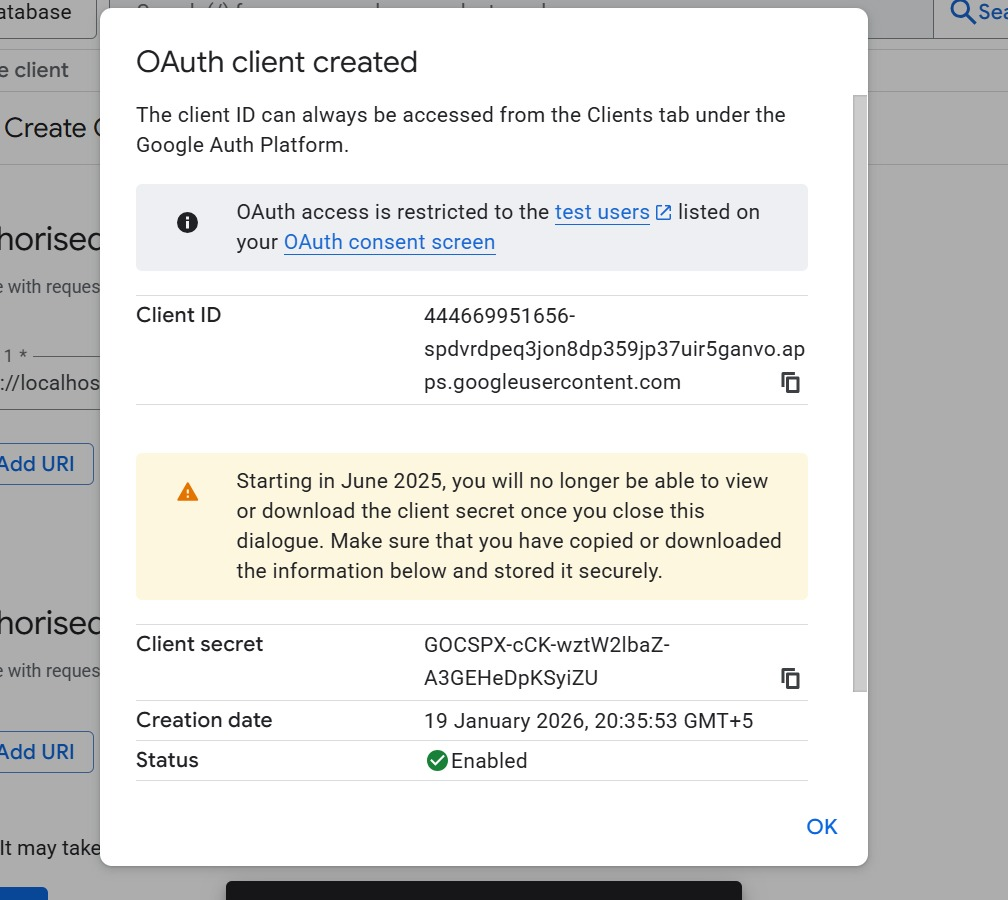
\includegraphics[width=0.9\textwidth]{uploaded_image_3_1768840342969.png}
    \caption{Google OAuth Client Setup}
\end{figure}

\subsection{Google Cloud Credentials}
Overview of active API credentials.
\begin{figure}[H]
    \centering
    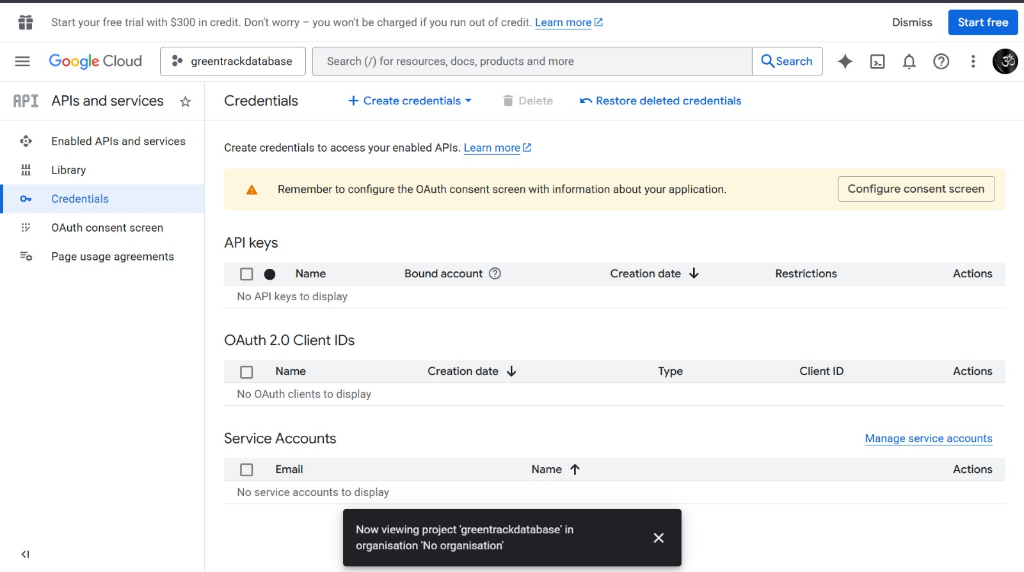
\includegraphics[width=0.9\textwidth]{uploaded_image_4_1768840342969.png}
    \caption{Google Cloud Config}
\end{figure}

\section{Application Interface}

\subsection{Live Feed Dashboard}
The central hub for community activity.
\begin{figure}[H]
    \centering
    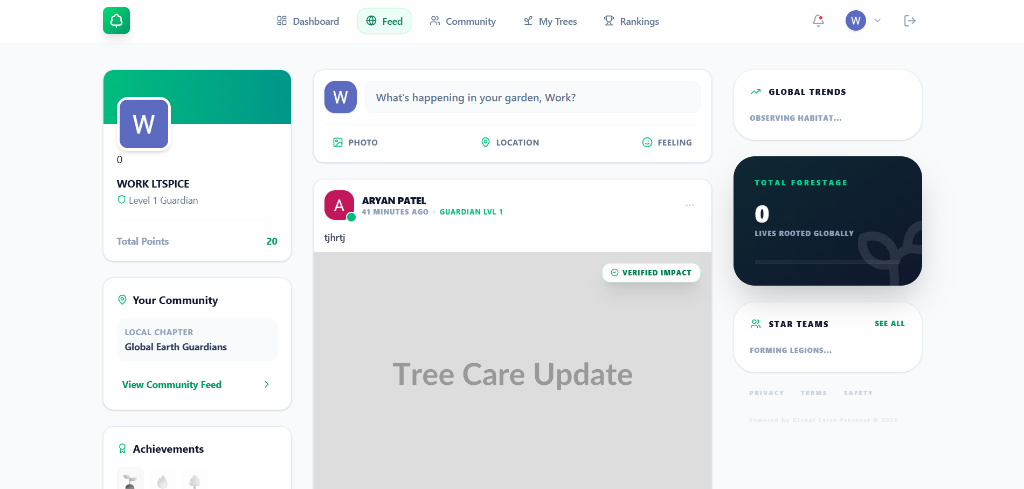
\includegraphics[width=0.9\textwidth]{uploaded_image_0_1768840595964.png}
    \caption{Live Feed Dashboard}
\end{figure}

\subsection{My Forest Inventory}
Personalized view of planted trees.
\begin{figure}[H]
    \centering
    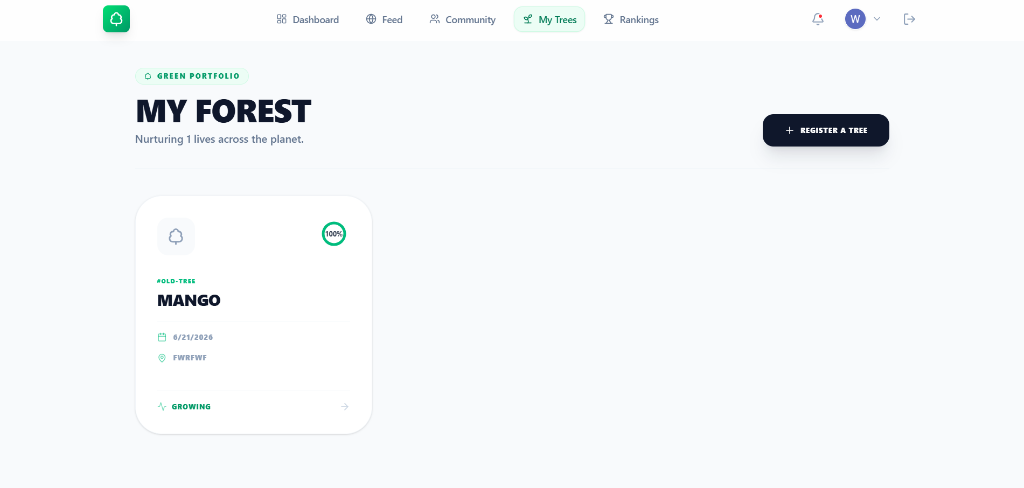
\includegraphics[width=0.9\textwidth]{uploaded_image_1_1768840595964.png}
    \caption{My Forest Inventory}
\end{figure}

\subsection{Global Leaderboard}
Rankings of top planters and teams.
\begin{figure}[H]
    \centering
    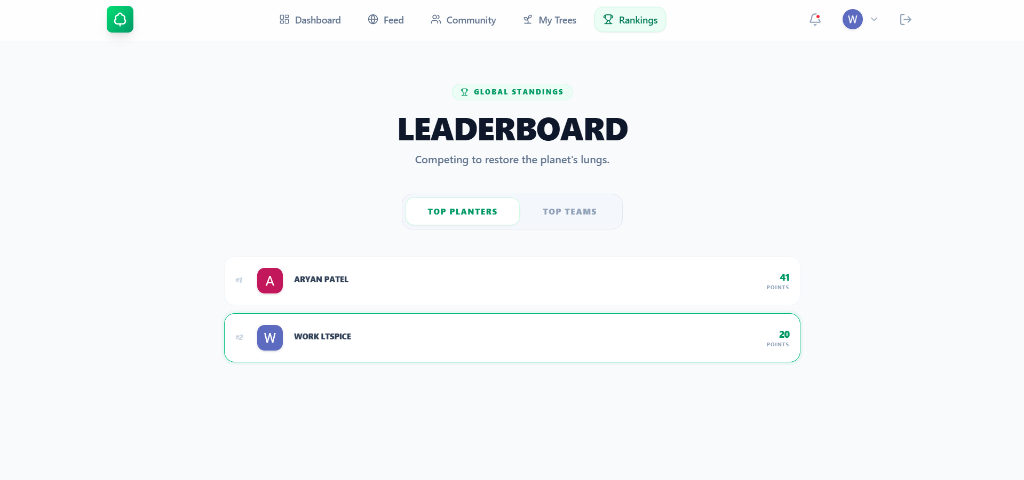
\includegraphics[width=0.9\textwidth]{uploaded_image_2_1768840595964.png}
    \caption{Global Leaderboard}
\end{figure}

\subsection{User Profile and Achievements}
User stats and gathered badges.
\begin{figure}[H]
    \centering
    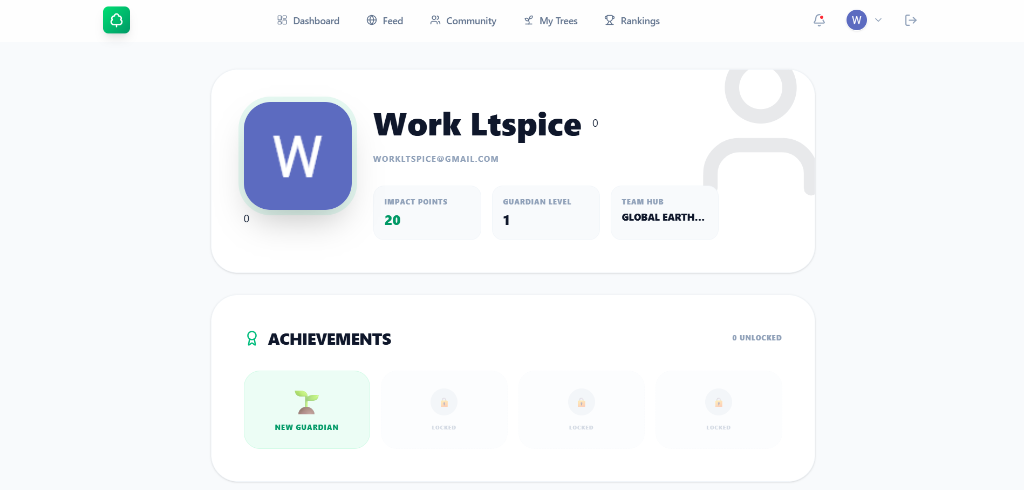
\includegraphics[width=0.9\textwidth]{uploaded_image_3_1768840595964.png}
    \caption{User Profile Page}
\end{figure}

\end{document}
